\chapter{Implementasi dan Pengujian}
\label{chap:implementation}
Pada bagian ini akan dijelaskan mengenai lingkungan implementasi perangkat keras maupun perangkat lunak. Serta implementasi basisdata BI \textit{tool} beserta tampilan antar muka. Terakhir akan dibahas mengenai pengujian pada perangkat lunak ini.
\section{Lingkungan Implementasi}
\subsection{Lingkungan Perangkat Keras}
Dalam mengembangakan perangkat ini, digunakan spesifikasi perangkat keras sebagai berikut:
\begin{itemize}
	\item \text{Processor} : Intel Core i7 2.4 Ghz
	\item \textit{Memory} : 8 GB
	\item \textit{Hardisk} : 640 GB
	\item VGA : Nvidia GeForce 540M
	\item \textit{keyboard} dan \textit{mouse standard}
\end{itemize}

\subsection{Lingkungan Perangkat Lunak}
Untuk pengembangan perangkat lunak BI \textit{tool}, digunakan spesifikasi sebagai berikut:
\begin{itemize}
	\item \textit{Tools:} ODOO 8.0-20141128
	\item Bahasa Pemograman Phyton 2.7
	\item \textit{Database management system} PosgreSQL 9.3
	\item \textit{Operating system}: windows 8
\end{itemize}

\section{Implementasi Tabel Basisdata}
\subsection{Tabel Basisdata ETL dan Bisnis}
Berikut implementasi tabel basisdata yang terlibat langsung dalam proses ETL beserta pendukungnnya.
\begin{itemize}
	\item Tabel ba\_business\\
	Tabel ini digunakan untuk mencatat semua bisnis yang menggunakan perangkat lunak ini. Selain itu , agar dapat \textit{multicompany/multiclient}.
	
	\begin{figure}[H]
	\centering
	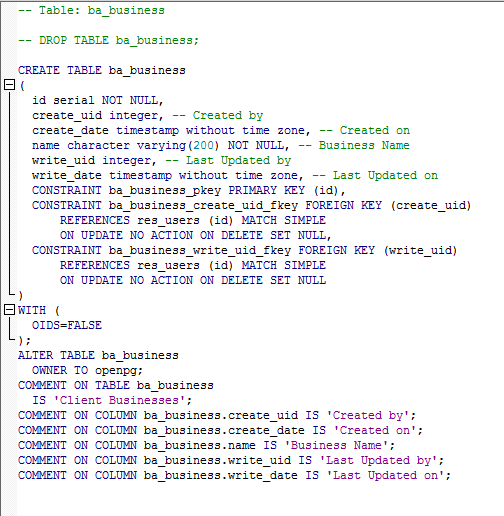
\includegraphics[scale=0.5]{Gambar/tabel-ba-business}
	\caption{Implementasi tabel ba\_business}
	\end{figure}

	\item Tabel ba\_etl\_header\\
	Tabel ini mencatat proses ETL yang ada di bawah perusahaan/bisnis yang ada.
	\begin{figure}[H]
	\centering
	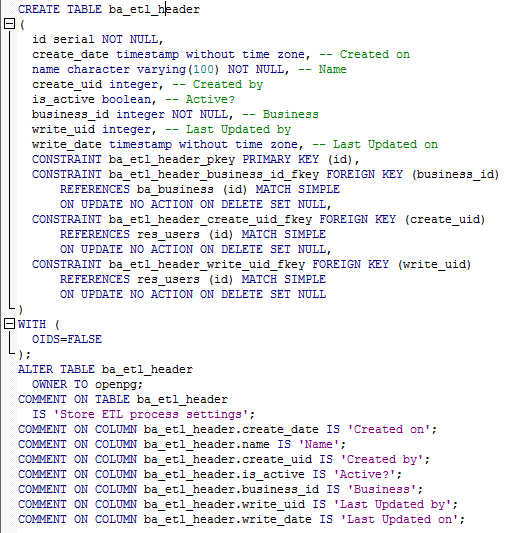
\includegraphics[scale=0.5]{Gambar/tabel-ba-etl-header}
	\caption{Implementasi tabel ba\_etl\_header}
	\end{figure}
	
	\item Tabel ba\_etl\_detail\\
	Tabel ini mencata detail dari setiap proses ETL dibawah perusahaan/bisnis. 
	\begin{figure}[H]
	\centering
	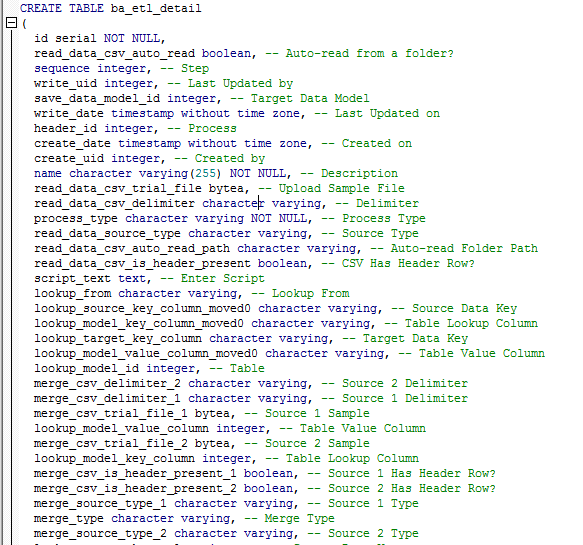
\includegraphics[scale=0.5]{Gambar/tabel-ba-etl-detail}
	\caption{Implementasi tabel ba\_etl\_detail}
	\end{figure}
	
	\begin{figure}[H]
	\centering
	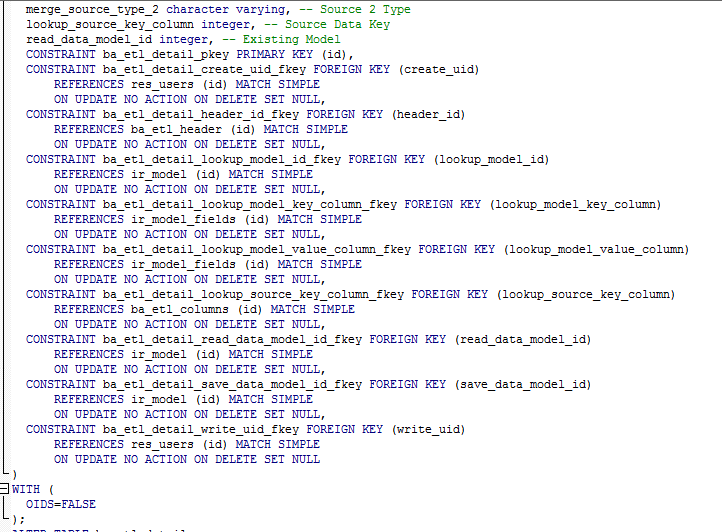
\includegraphics[scale=0.5]{Gambar/tabel-ba-etl-detail2}
	\caption{Implementasi tabel ba\_etl\_detail2}
	\end{figure}

\begin{figure}[H]
	\centering
	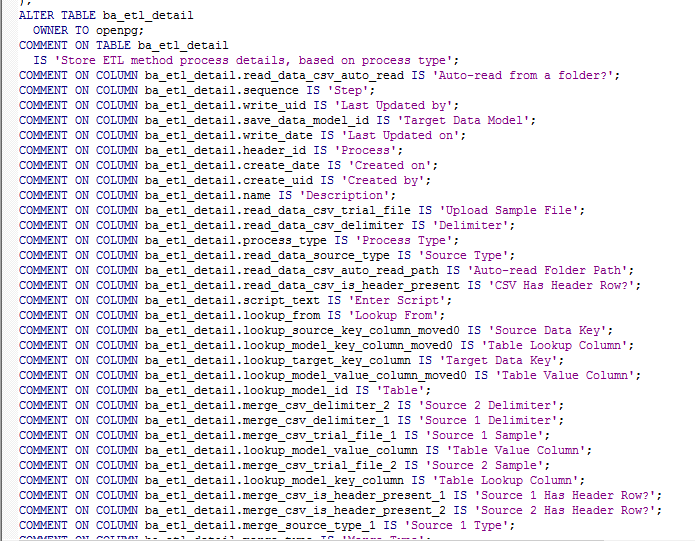
\includegraphics[scale=0.5]{Gambar/tabel-ba-etl-detail3}
	\caption{Implementasi tabel ba\_etl\_detail3}
	\end{figure}

	\item Tabel basisdata ba\_etl\_columns\\
	Tabel ini berfungsi menyimpan kolom-kolom yang terlibat dalam proses ETL, baik dari sumber data maupun yang ditambahkan di tengah proses
	\begin{figure}[H]
		\centering
		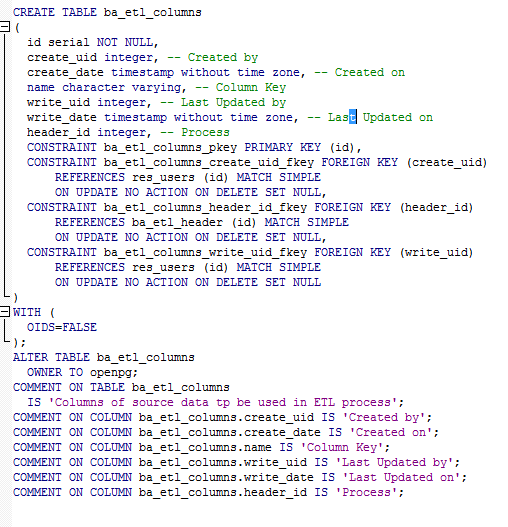
\includegraphics[scale=0.5]{Gambar/tabel-ba-etl-columns}
		\caption{Implementasi tabel ba\_etl\_columns}
		\end{figure}
	
	\item Tabel basisdata ba\_etl\_columns\_mapping\\
	Tabel ini menyimpan detail \textit{mapping} kolom dari data \textit{input} ke \textit{output}.
	\begin{figure}[H]
		\centering
		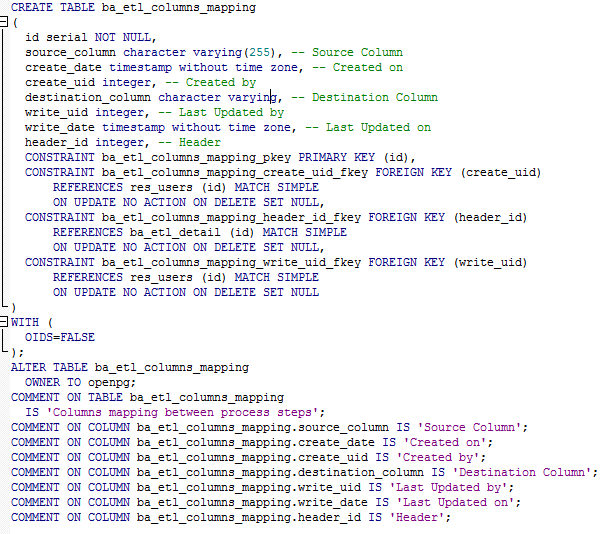
\includegraphics[scale=0.5]{Gambar/tabel-ba-etl-columns-mapping}
		\caption{Implementasi tabel ba\_etl\_columns\_mapping}
		\end{figure}
	
	\item Tabel basisdata ba\_etl\_format\_data\_lines\\ Tabel ini menyimpan detil informasi dari setiap kolom khusus tipe ETL Format Data.
	\begin{figure}[H]
		\centering
		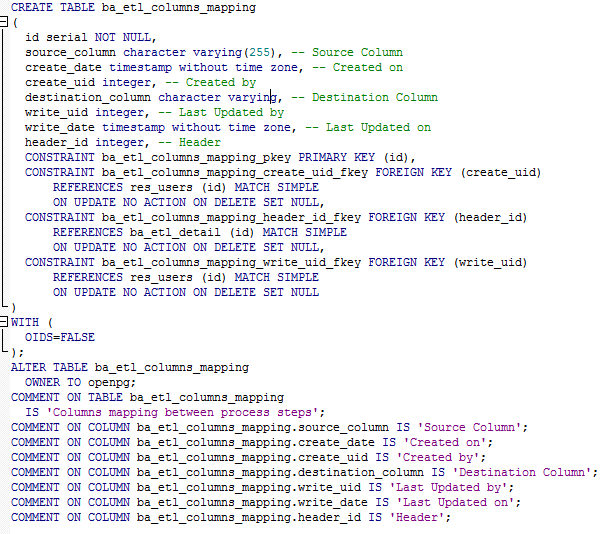
\includegraphics[scale=0.5]{Gambar/tabel-ba-etl-columns-mapping}
		\caption{Implementasi tabel ba\_etl\_columns\_mapping}
		\end{figure}
	
	\item Tabel basisdata ba\_etl\_sort\_data\_columns\\
	Tabel ini menyimpan detail kolom dan arah sorting khusus tipe ETL \textit{Sort Data}
	\begin{figure}[H]
		\centering
		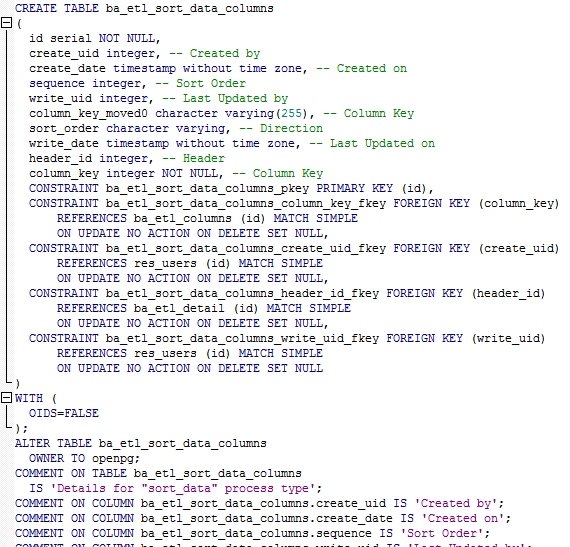
\includegraphics[scale=0.5]{Gambar/tabel-ba-etl-sort-data-columns}
		\caption{Implementasi tabel ba\_etl\_sort\_data\_columns}
		\end{figure}
		
		\item Tabel basisdata ba\_etl\_derived\_column\_lines\\
		Tabel ini menyimpan detail formula untuk menghasilkan \textit{derived column} khusus tipe ETL \textit{Derived Column}.
		\begin{figure}[H]
		\centering
		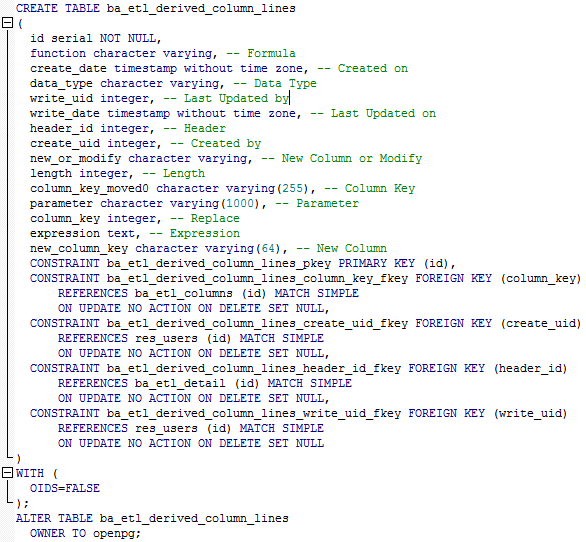
\includegraphics[scale=0.5]{Gambar/tabel-ba-etl-dericed-column-lines}
		\caption{Implementasi tabel ba\_etl\_derived\_column\_lines}
		\end{figure}
		
		\item Tabel basisdata ba\_etl\_lookup\_fixed\_lines\\
		Tabel ini menyimpan pilihan \textit{lookup} yang diambil dari himpan pilihan \textit{fixed}. Khusus tipe ETL \textit{lookup}.
		\begin{figure}[H]
		\centering
		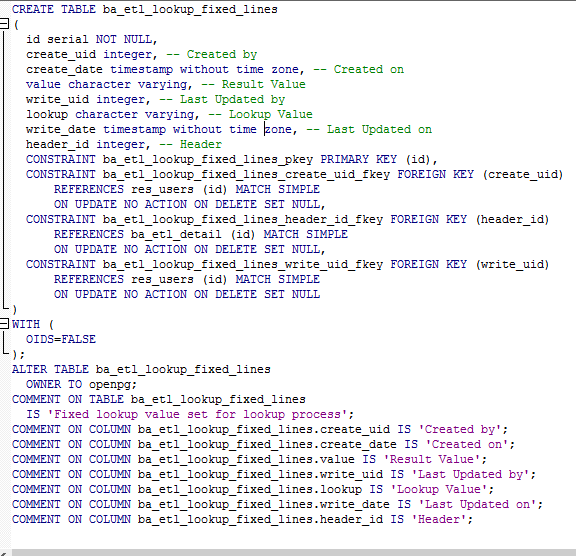
\includegraphics[scale=0.5]{Gambar/tabel-ba-etl-lookup-fixed-lines}
		\caption{Implementasi tabel ba\_etl\_lookup\_fixed\_lines}
		\end{figure}
		
		\item Tabel basisdata ba\_etl\_save\_data\_columns\\
		Tabel ini menyimpan \textit{mapping} kolom antara hasil proses dengan \textit{field} di tabel. Khusus tipe ETL \textit{Save Data} 
		\begin{figure}[H]
		\centering
		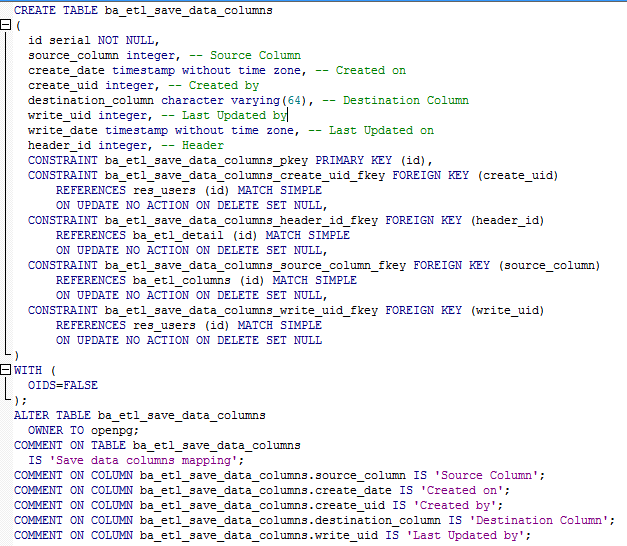
\includegraphics[scale=0.5]{Gambar/tabel-ba-etl-save-data-columns}
		\caption{Implementasi tabel ba\_etl\_save\_data\_columns}
		\end{figure}
		
		\item Tabel basisdata ba\_etl\_lookup\_model\_mappings\\
		Tabel ini menyimpan \textit{lookup} dari tabel lain, tabel ini menampung pasangan \textit{field} di data proses dengan yang di tabel lookup. Khusus tipe ETL \textit{lookup}
		\begin{figure}[H]
		\centering
		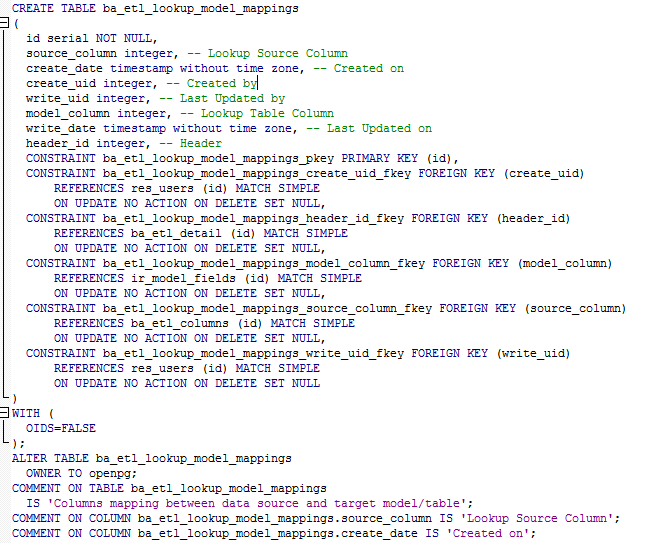
\includegraphics[scale=0.5]{Gambar/tabel-ba-etl-lookup-model-mappings}
		\caption{Implementasi tabel ba\_etl\_lookup\_model\_mappings}
		\end{figure}
		
		\item Tabel basisdata ba\_etl\_merge\_columns1\\
		Tabel ini menyimpan informasi \textit{merge} dari sumber pertama. Khusus tipe ETL \textit{Merge}
		\begin{figure}[H]
		\centering
		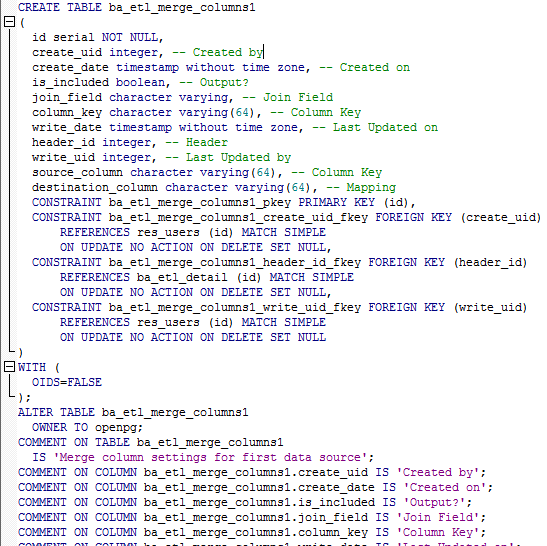
\includegraphics[scale=0.5]{Gambar/tabel-ba-etl-merge-columns1}
		\caption{Implementasi tabel ba\_etl\_merge\_columns1}
		\end{figure}
		
		\item Tabel basisdata ba\_etl\_merge\_columns2\\
		Tabel ini menyimpan informasi \textit{merge} dari sumber kedua. Khusus tipe ETL \textit{Merge}
		\begin{figure}[H]
		\centering
		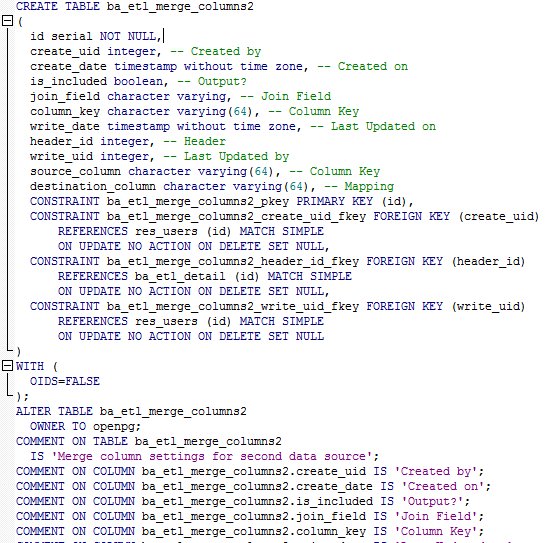
\includegraphics[scale=0.5]{Gambar/tabel-ba-etl-merge-columns2}
		\caption{Implementasi tabel ba\_etl\_merge\_columns2}
		\end{figure}
		
		\item Tabel basisdata ba\_etl\_aggregate\_columns\\
		Tabel ini menyimpan detail informasi proses aggregate khusus tipe ETL \textit{aggregate}.
		\begin{figure}[H]
		\centering
		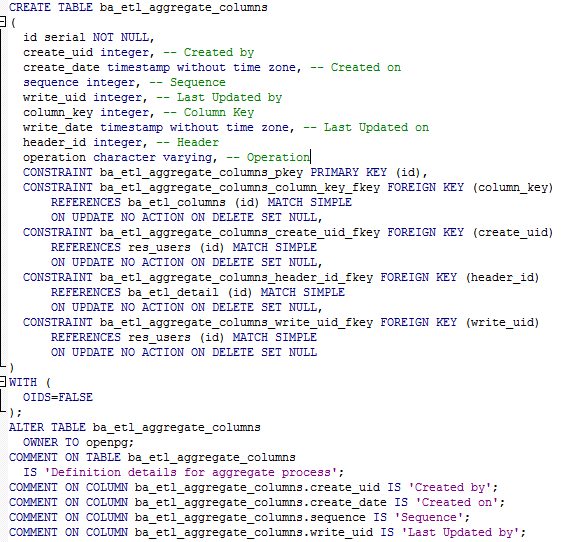
\includegraphics[scale=0.5]{Gambar/tabel-ba-etl-aggregate-columns}
		\caption{Implementasi tabel ba\_etl\_aggregate\_columns}
		\end{figure}
	\end{itemize}
	
	\section{Implementasi Kode Program Phyton}
	Berikut ini sisipan kode program perangkat lunak BI \textit{tool}
	\begin{enumerate}
		\item Kode Program \textit{load} kolom dari \textit{source}\\
		\begin{figure}[H]
		\centering
		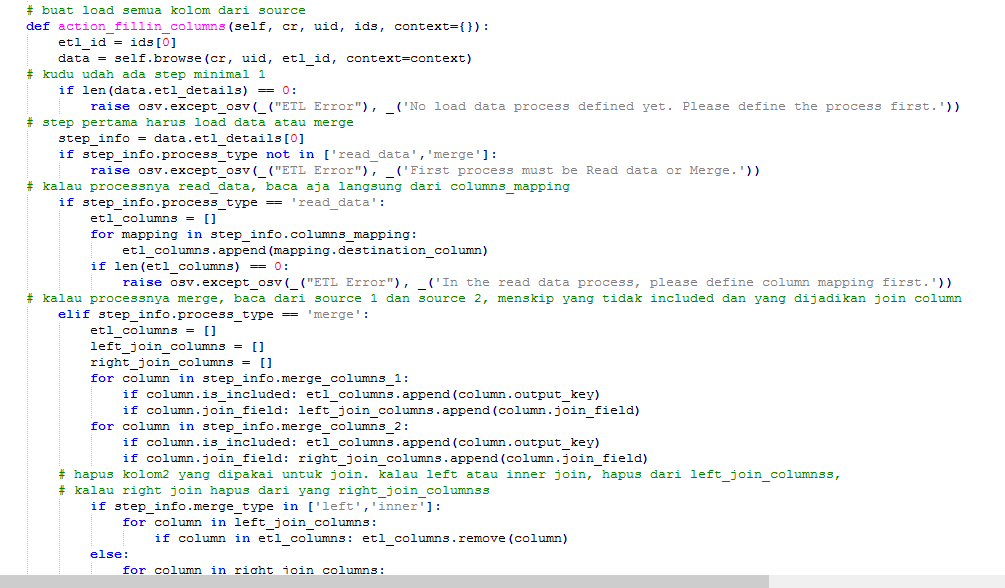
\includegraphics[scale=0.5]{Gambar/kode-load}
		\caption{kode program \textit{load columns from source}}
		\end{figure}
	\item Kode Program untuk \textit{mapping column}
	\begin{figure}[H]
		\centering
		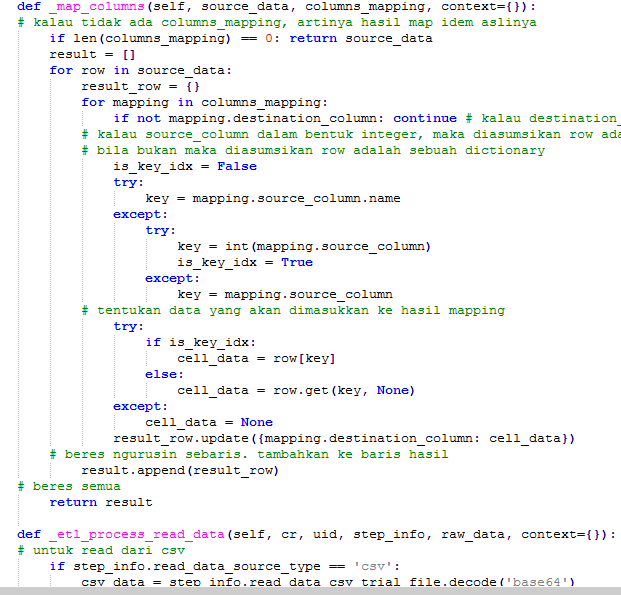
\includegraphics[scale=0.5]{Gambar/kode-mapping}
		\caption{Kode Program untuk \textit{mapping column}}
		\end{figure}
	\end{enumerate}
	
	\section{Implementasi Antar Muka}
	\subsection{Implementasi Antar Muka untuk \textit{Business}}
	\begin{itemize}
		\item Buat Bisnis Baru\\
		Halaman ini digunakan ketika pertama perusahaan akan membuat bisnis baru sebelum masuk pada proses ETL.
		\begin{figure}[H]
		\centering
		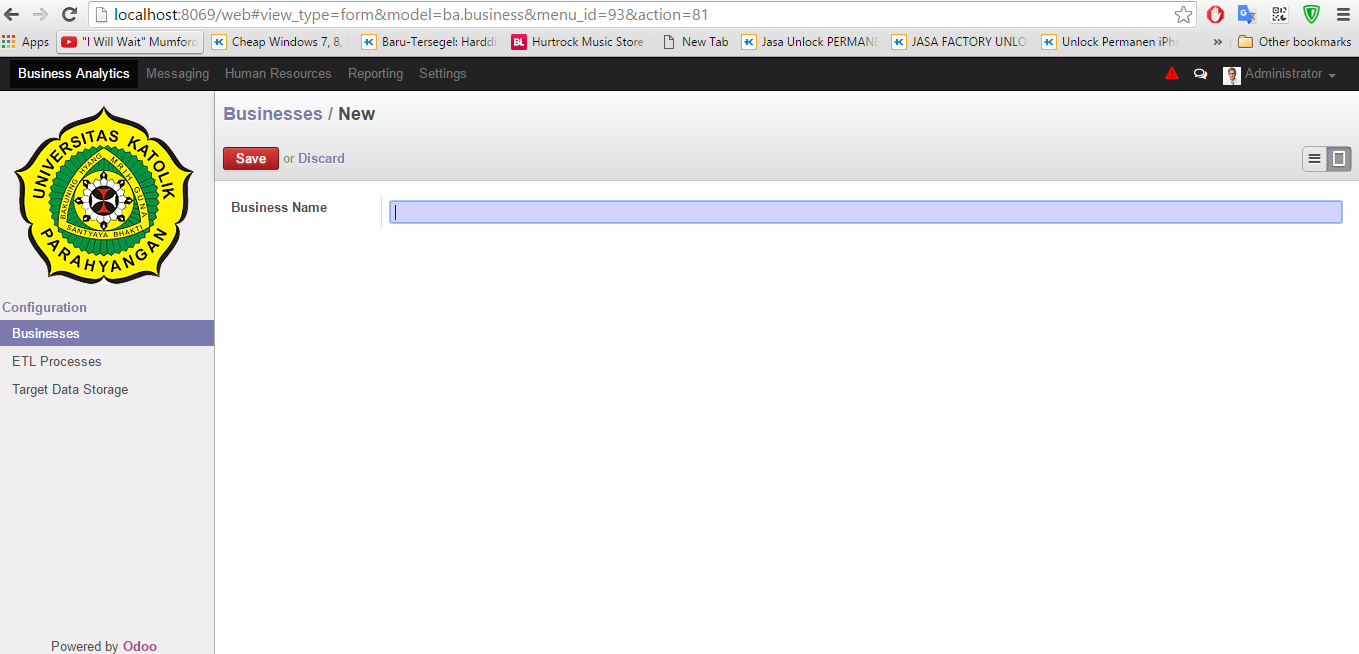
\includegraphics[scale=0.4]{Gambar/tampilan-business}
		\caption{Tampilan untuk membuat bisnis baru}
		\end{figure}
	\end{itemize}
	
	\subsection{Implementasi Antar Muka untuk Proses ETL}
	\begin{itemize}
		\item Membuat Proses ETL Baru\\
		Halaman ini digunakan ketika membuat proses ETL baru.
		\begin{figure}[H]
		\centering
		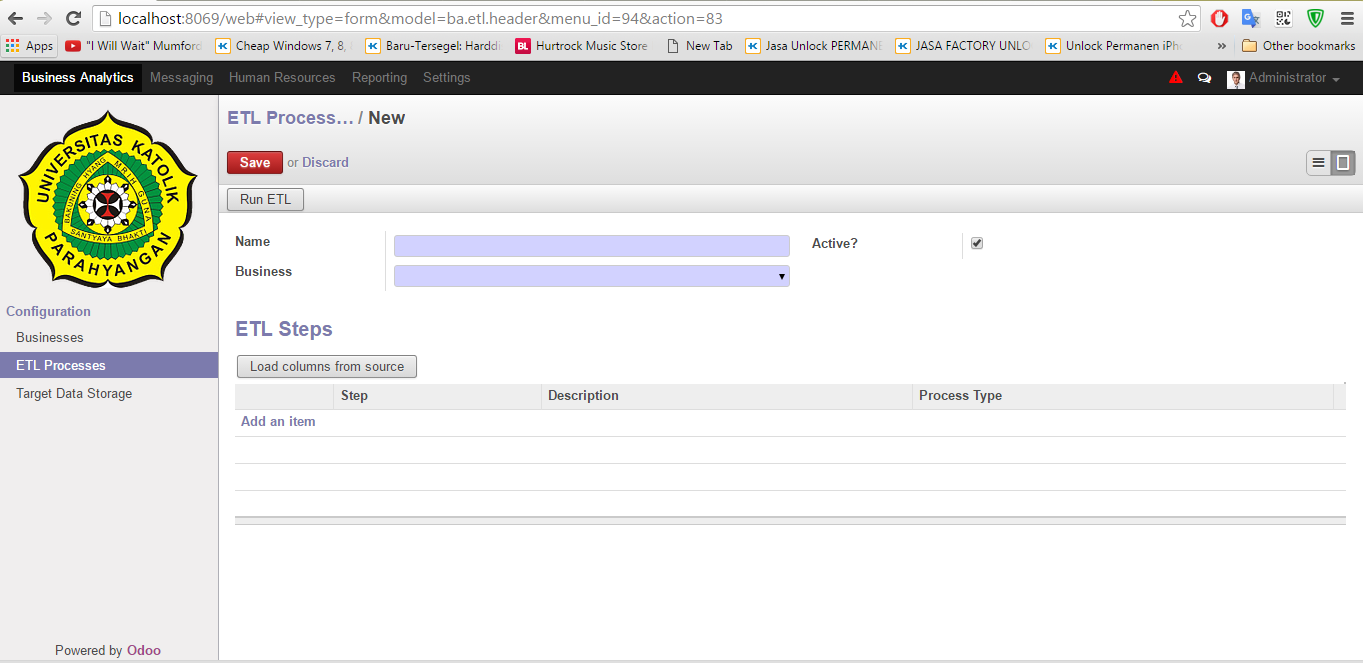
\includegraphics[scale=0.4]{Gambar/tampilan-etl-baru}
		\caption{Tampilan untuk membuat ETL baru}
		\end{figure}
		
		\item \textit{Upload Source}\\
		Halaman ini digunakan ketika pengguna meng-\textit{upload data source}.
		
		\begin{figure}[H]
		\centering
		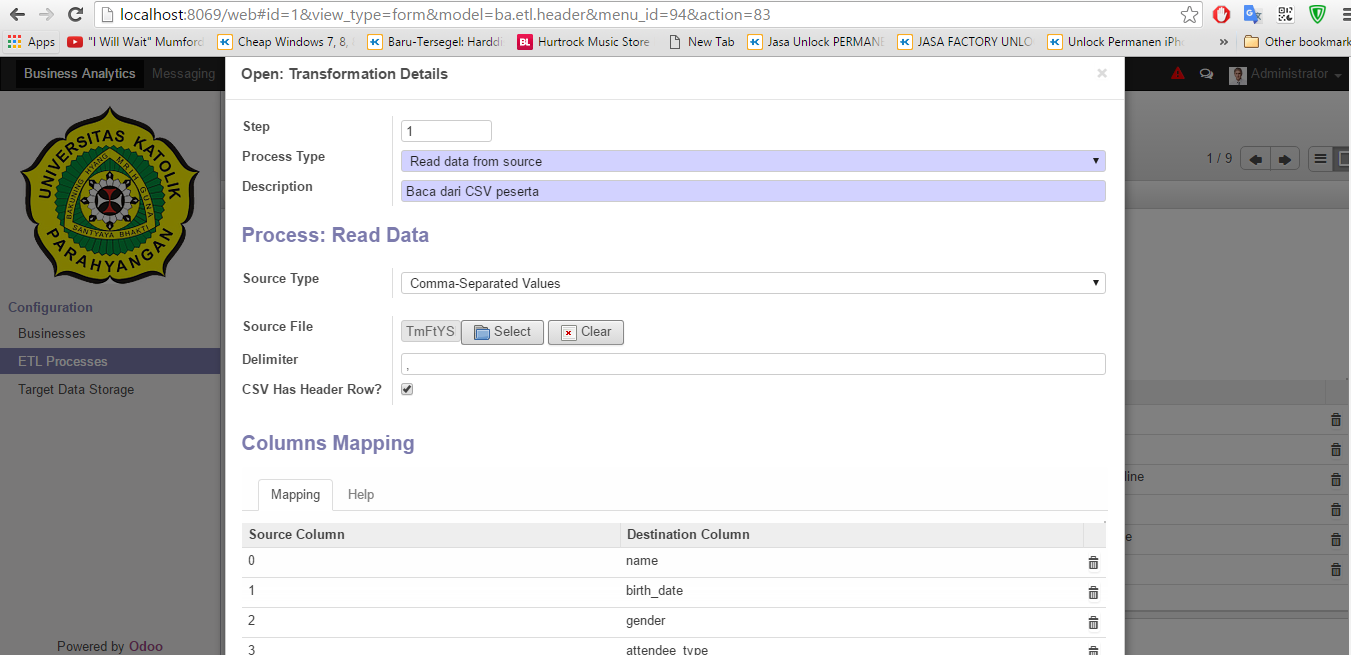
\includegraphics[scale=0.4]{Gambar/tampilan-upload-source}
		\caption{Tampilan untuk \textit{upload source}}
		\end{figure}
		
		\item \textit{Determine Data Types and Format}\\
		Halaman ini memudahkan pengguna untuk menentukan format dan tipe data pada \textit{source}.
		
		\begin{figure}[H]
		\centering
		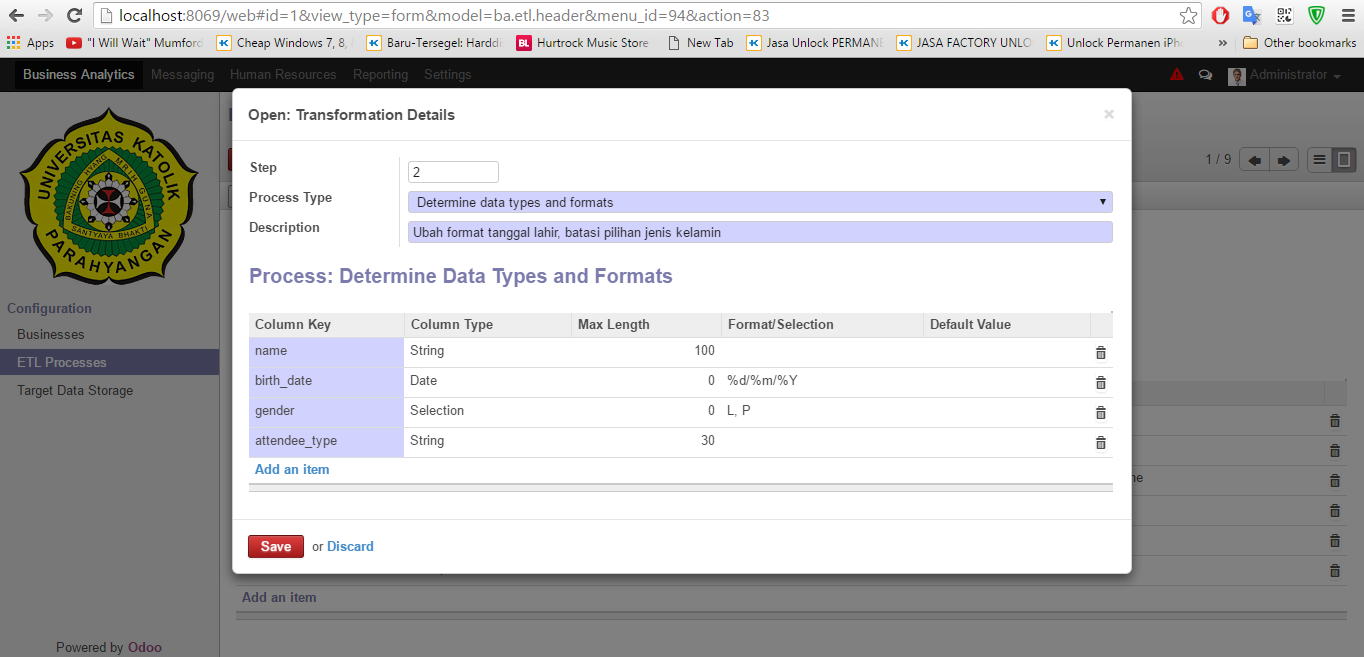
\includegraphics[scale=0.4]{Gambar/tampilan-ubah-data}
		\caption{Tampilan untuk ubah data dan format data}
		\end{figure}
	
	\item Menerapkan Skrip Phyton\\
	Halaman ini dapat digunakan pengguna ketika akan menerapkan kode phyton untuk memodifikasi \textit{source}.
	
	\begin{figure}[H]
		\centering
		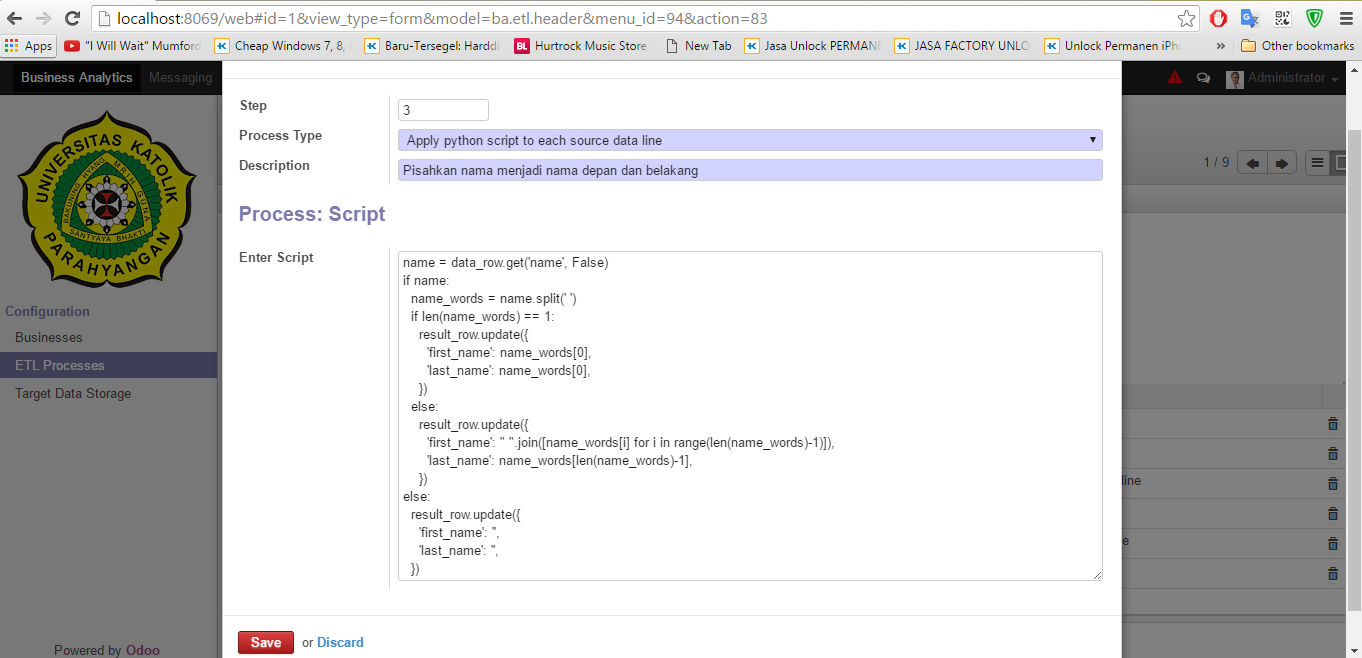
\includegraphics[scale=0.4]{Gambar/tampilan-menerapkan-skrip-phyton}
		\caption{Tampilan untuk menerapkan skrip phyton}
		\end{figure}
		
		\item Tampilan \textit{Lookup} dengan \textit{Existing Table}
		Halaman ini digunakan ketika pengguna ingin melakukan lookup dengan tabel lain yang sudah dimasukan terlebih dahulu dalam \textit{database}
		\begin{figure}[H]
		\centering
		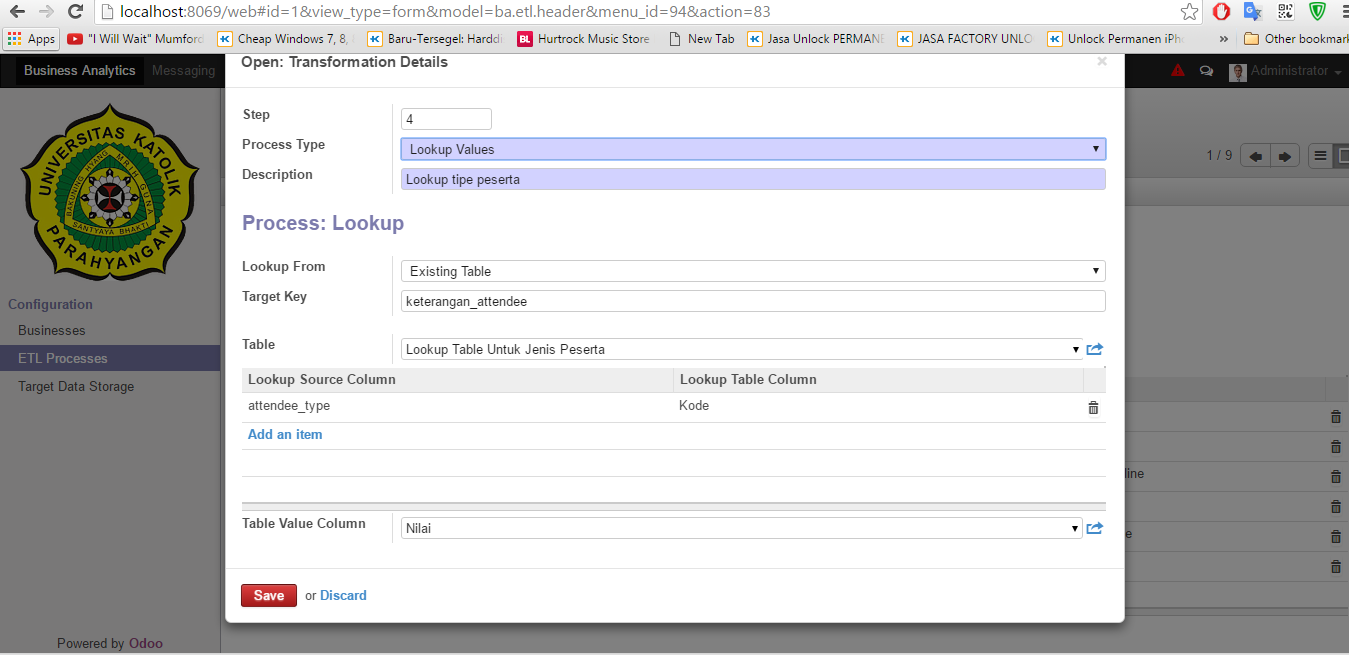
\includegraphics[scale=0.4]{Gambar/tampilan-lookup-existing-table}
		\caption{Tampilan untuk \textit{lookup} dari \textit{existing table}}
		\end{figure}
		
		\item Tampilan \textit{Lookup} dengan \textit{Values Below}
		Halaman ini digunakan ketika pengguna ingin melakukan lookup dengan nilai \textit{lookup} dan hasil yang dimasukan langsung oleh pengguna
		\begin{figure}[H]
		\centering
		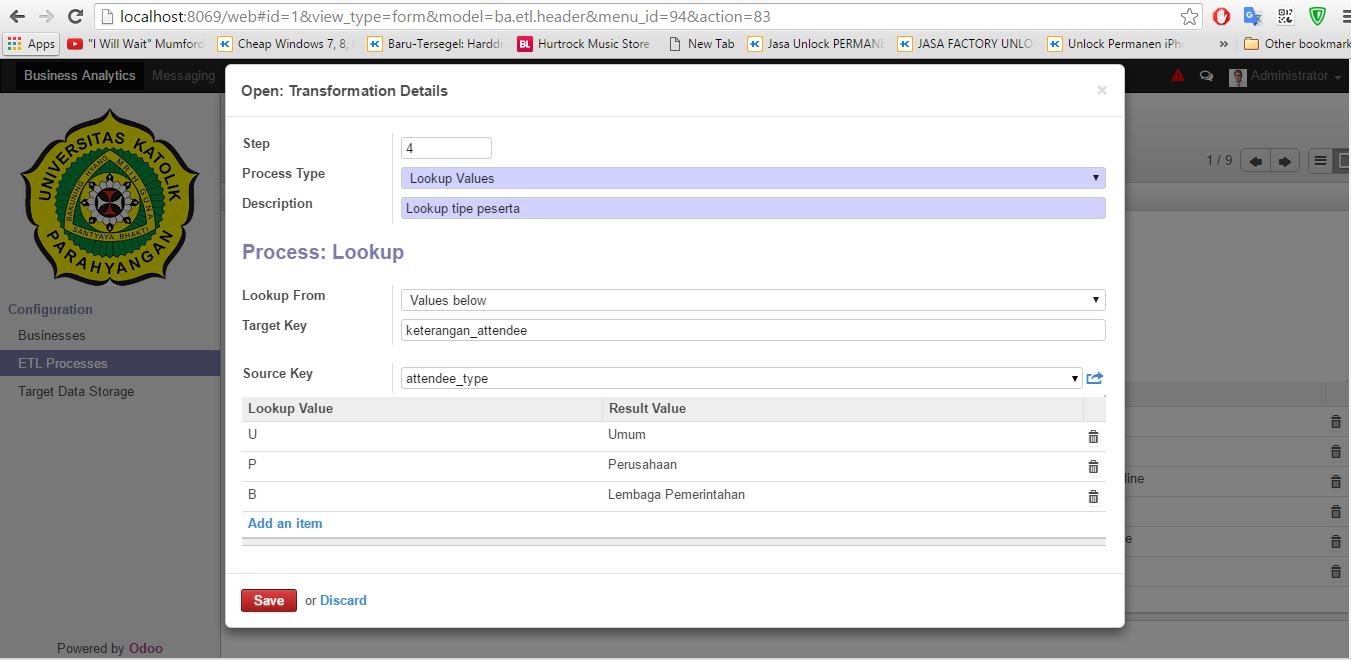
\includegraphics[scale=0.4]{Gambar/tampilan-lookup-values-below}
		\caption{Tampilan untuk \textit{lookup} dari \textit{value} yang dituliskan pengguna}
		\end{figure}
		
		\item Menambah atau memodifikasi kolom yang tersedia\\
		Halaman ini digunakan ketika pengguna ingin menambahkan kolom atau memodifikasi kolom yang tersedia.
		
		\begin{figure}[H]
		\centering
		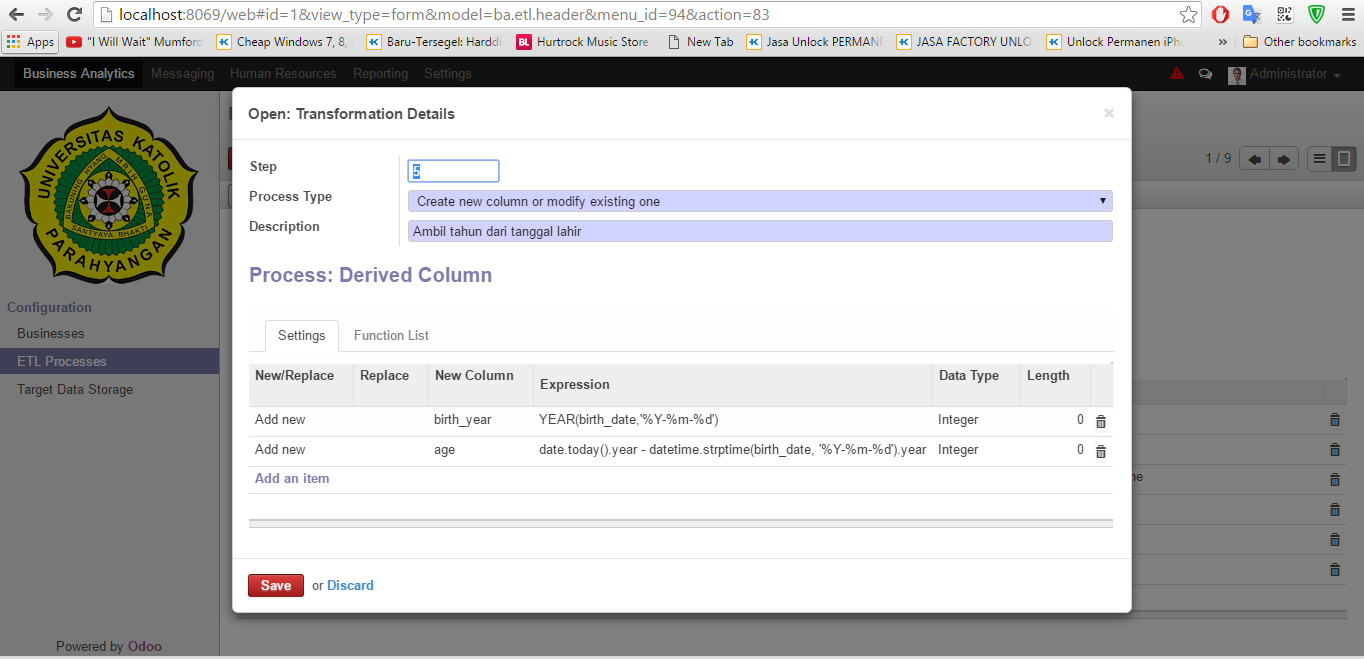
\includegraphics[scale=0.4]{Gambar/tampilan-menambah-kolom}
		\caption{Tampilan untuk menambah atau memodifikasi kolom}
		\end{figure}
		
		
		\item \textit{Merging} dua \textit{data source}\\
		Halaman ini digunakan ketika pengguna ingin menggabungkan dua \textit{data source} menjadi satu.
		
		\begin{figure}[H]
		\centering
		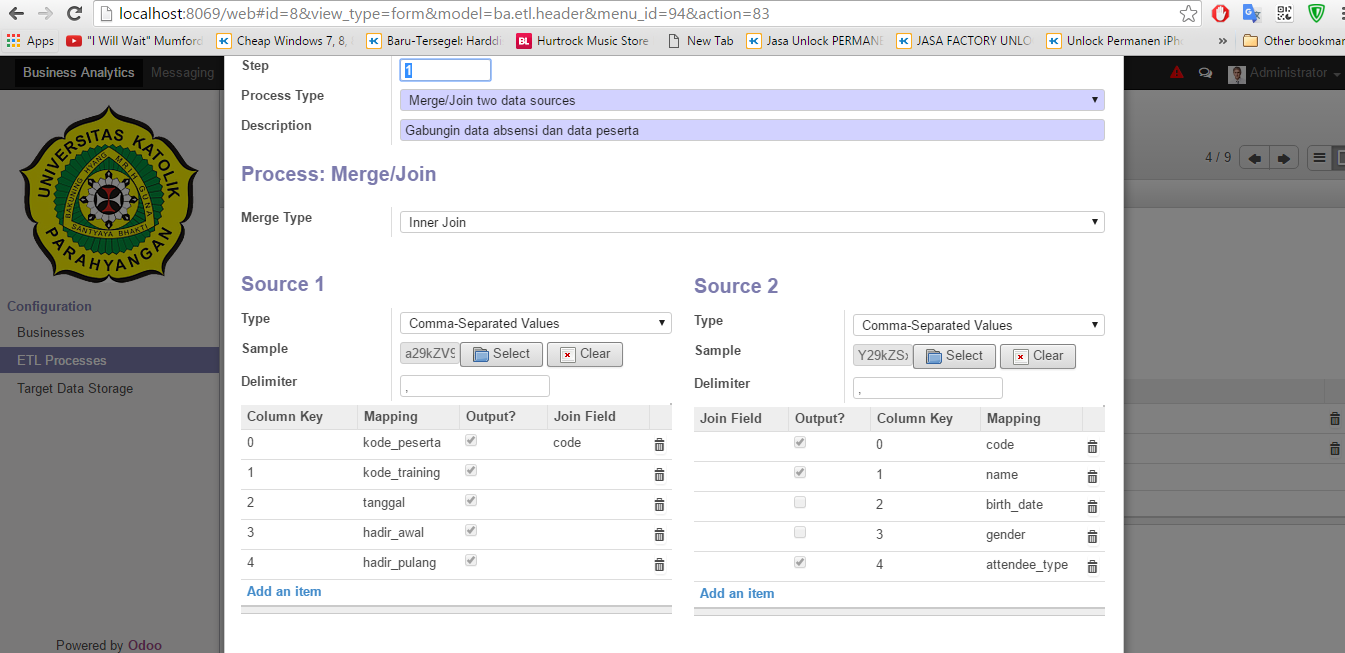
\includegraphics[scale=0.4]{Gambar/tampilan-merge}
		\caption{Tampilan untuk \textit{merging} dua \textit{source}}
		\end{figure}
		
		\item Melakukan \textit{Sorting data}\\
		Halaman ini digunakan ketika pengguna ingin melakukan \textit{sorting data} .
		\begin{figure}[H]
		\centering
		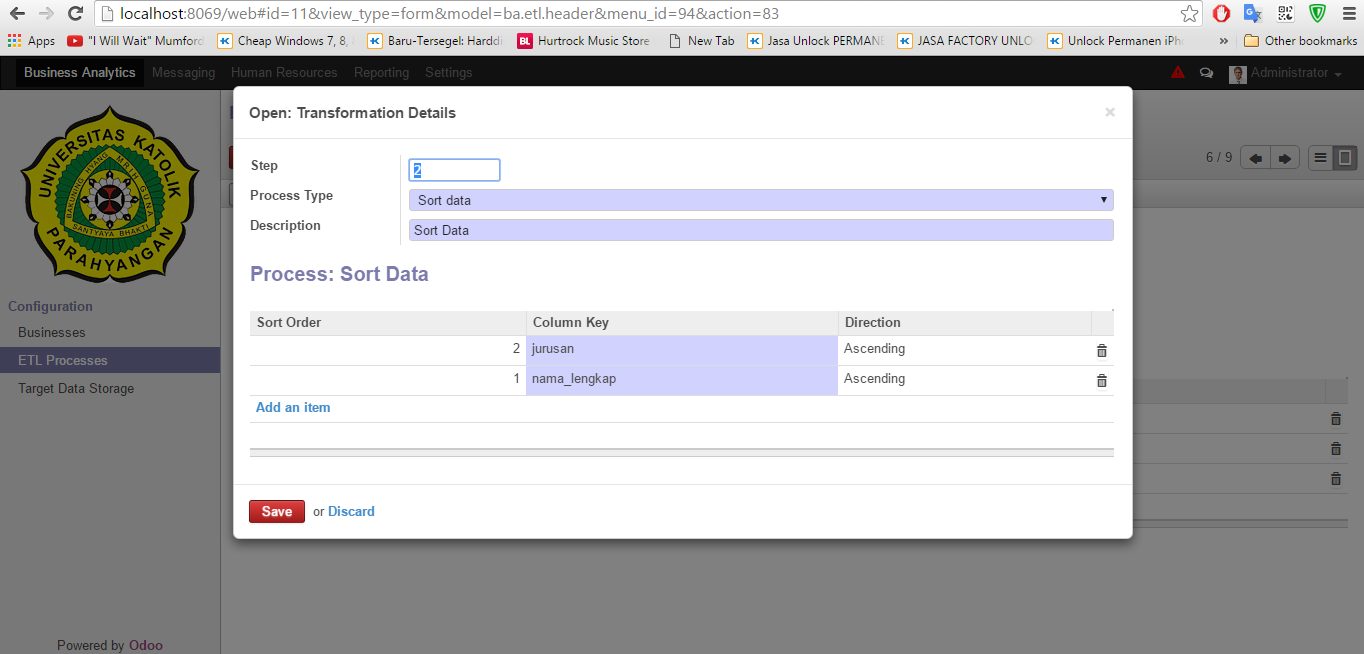
\includegraphics[scale=0.4]{Gambar/tampilan-sort-data}
		\caption{Tampilan untuk melakukan \textit{sort}}
		\end{figure}
		
		\item Melakukan Agregat\\
		Tampilan ini digunakan pengguna ketika akan melakukan agregat terhadap \textit{source}
		\begin{figure}[H]
		\centering
		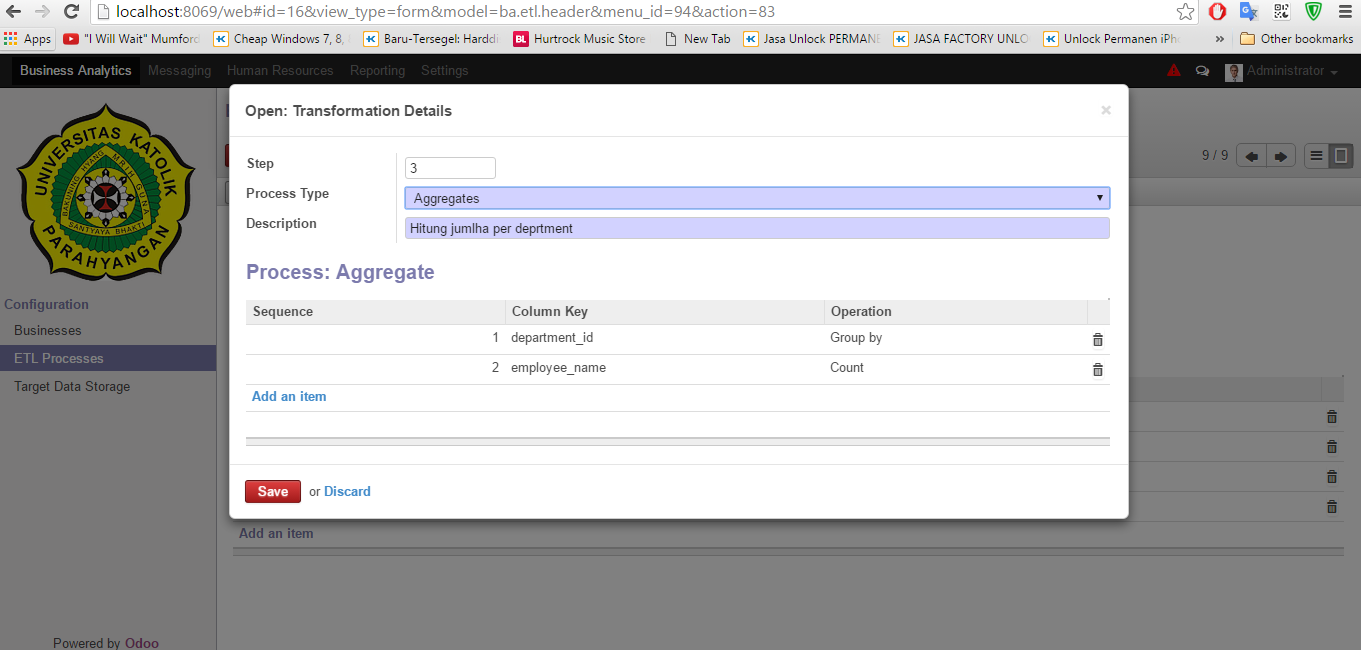
\includegraphics[scale=0.4]{Gambar/tampilan-agregat}
		\caption{Tampilan untuk melakukan agregat}
		\end{figure}
		
		\item Menyimpan ke \textit{database}\\
		Halaman ini digunakan ketika pengguna ingin menyimpan hasil ETL kedalam \textit{database}.

		\begin{figure}[H]
		\centering
		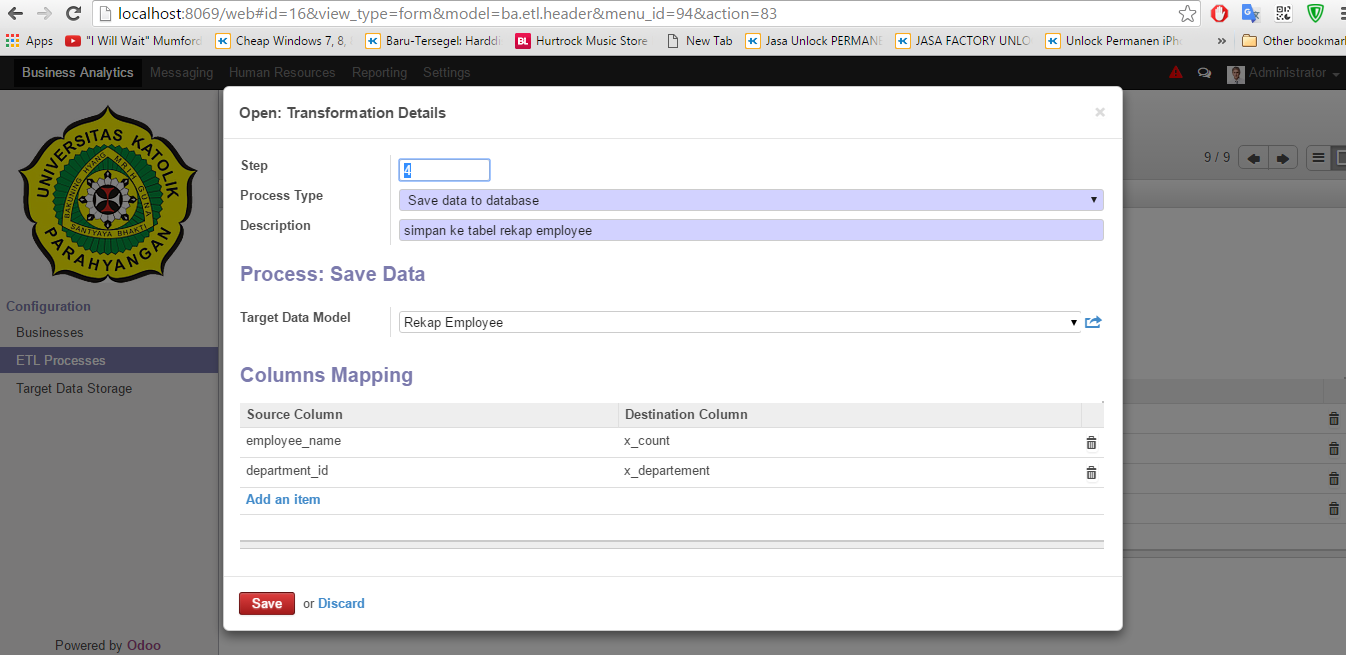
\includegraphics[scale=0.4]{Gambar/tampilan-simpan-database}
		\caption{Tampilan untuk menyimpan kedalam \textit{database}}
		\end{figure}
	\end{itemize}
	
	\section{Pengujian}
	Pada subab ini akan dibahas mengenai pengujian terhadap perangkat lunak ini sehingga dapat mengukur seberapa baik performansinya. berikut ini merupakan \textit{sample data customer} yang akan digunakan.
	
	\begin{table}[H]
	\centering
		\caption{Contoh Tabel \textit{customer}}
		\begin{tabular}{ | c | c| c | c | p{2cm} | p{2cm} | c |}
			\hline
				CIF & BRANCHCODE & GENDER & AGE & MARITAL STATUS & INCOME LEVEL & TENURE \\ \hline \hline
			1000000&ID0010096&2&15131&0&1&1175 \\ \hline 
			1000043&ID0010075&2&14972&1&1&1175 \\ \hline
			1000044&ID0010049&2&13401&1&1&1175 \\ \hline
			1000056&ID0010049&1&18992&1&1&1175 \\ \hline
			1000059&ID0010038&2&20871&1&1&1175 \\ \hline
			1000064&ID0010049&2&20852&1&1&1175 \\ \hline
			1000067&ID0010038&1&15728&1&1&1175 \\ \hline
			1000068&ID0010049&1&16176&1&1&1175 \\ \hline
			1000069&ID0010026&1&19069&1&1&1175 \\ \hline
			1000075&ID0010038&1&11279&1&1&1175 \\ \hline
			1000076&ID0010090&1&18562&1&1&1175 \\ \hline
			1000084&ID0010090&2&14490&1&1&1175 \\ \hline
			1000140&ID0010129&1&15216&1&1&1174 \\ \hline
			1000149&ID0010026&1&9566&0&1&1174 \\ \hline
			1000166&ID0010108&2&14100&1&6&1174 \\ \hline
			1000195&ID0010014&1&12617&0&3&1174 \\ \hline
			1000202&ID0010132&1&23236&1&1&1174 \\ \hline
			1000244&ID0010096&2&19106&1&2&1174 \\ \hline
			1000246&ID0010038&2&27964&1&1&1174 \\ \hline
		\end{tabular}
\end{table}

Hasil Pengujian fitur adalah sebagai berikut.
\begin{enumerate}
	\item \textit{Sort, Aggregate, Modify Existing one, Read Source, Save to Database}\\
	Hasil pengujian proses ETL dapat dilihat pada tabel dibawah ini.
	
	\begin{table}[H]
	\centering
		\caption{Tabel \textit{ba\_bussiness}}
		\begin{tabular}{ | c | p{3cm}| p{3cm}| p{3cm} | }
			\hline
				Hal yang diuji & Hasil yang diharapkan & Hasil Pengujian & Status \\ \hline \hline
			 \textit{Upload CSV} & Berhasil Melakukan \textit{upload} CSV & Berhasil Melakukan \textit{upload} CSV & OK \\ \hline
				Melakukan Sorting & Data tersorting berdasarkan \textit{branchcode} dan \textit{gender}. & Data tersorting berdasarkan \textit{branchcode} dan \textit{gender} & OK \\ \hline
				Melakukan Agregat & Hitung rata-rata umur per cabang per jenis kelamin & Data telah terhitung per rata-rata umur per cabang per jenis kelamin & OK \\ \hline
				Memodifikasi data & Ubah umur ke dalam satuan tahun & Umur telah berhasil diubah kedalam satuan tahun & OK \\ \hline
				Memodifikasi data & Ubah jenis kelamin menjadi P/L & Jenis kelamin menjadi P/L & OK \\ \hline
				Menyimpan ke \textit{database} & Simpan hasil ke \textit{database} & Data berhasil tersimpan ke \textit{database}& OK\\ \hline
			
		\end{tabular}
\end{table}
\end{enumerate}
	
